\chapter{State of the art Survey}

\section{Introduction}
This chapter introduce all the different technologies currently available which deal with anonymity and privacy. Some of the technologies are already commercially available and being used in the industry, while some are still in research phase. We will give a brief introduction for all of them and brief idea how they can be used.


\section{Technologies}

\begin{enumerate}
	\item Secure Multi-Party Computing
	\item Escrow Technologies
	\item Identity Management Systems
	\item Zero Knowledge Technologies
\end{enumerate}
\begin{figure}[h]
	\centering
	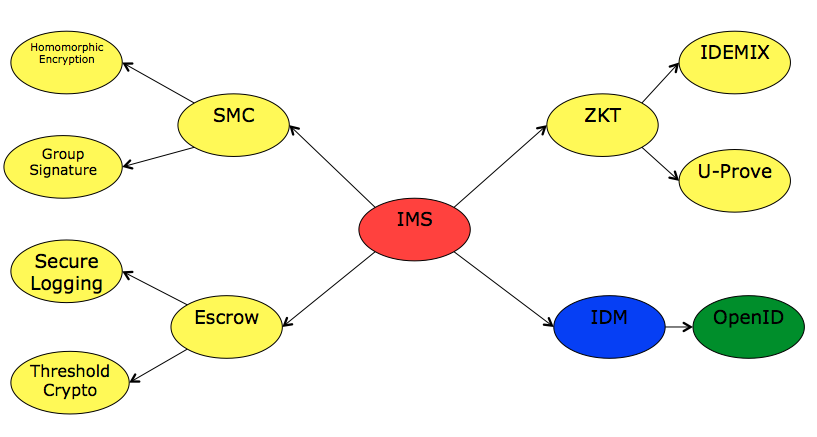
\includegraphics[width=\textwidth]{figures/Technologies}
	\caption{Technology Overview}
	\label{fig:Technologies}
\end{figure}

\section{Secure Multi-Party Computing}
These technologies are the ones which involve multiple parties to do computations. It is a subfield of cryptography which involves multiple parties getting an input and compute a joint function on them while keeping these inputs private. We basically looked at 2 technologies of interest here:
\subsection{Homomorphic Encryption}
Homomorphic encryption is a type of encryption where certain arithmetic operations can be performed on the ciphertext such that when the resultant ciphertext is decrypted, the decrypted text is same as the operations were performed on the plaintext. This is a new field of cryptography and is very useful where we need some parties to perform such operations without revealing the underlying data to those parties. Homomorphic encryption is also useful for chaining of different services without exposing data to any of those services.
\subsection{Group Signature}
A group signature is a scheme which allows a member of the group to sign the message on behalf of the group but anonymously. To outsiders the message has been signed by someone from the group but the exact identity of the person is now known. Also if the same member signs 2 different messages its not possible to know if the message is signed by the same member. There is a notion of group manager in these scheme. Group manager is someone who manages the membership to the group. He can add/remove members from the group, find out who actually signed the message from the group. This scheme is useful where only thing that needs to be validated is that a certain person is part of the group, but his real identity is not required.
\section{Escrow Technologies}
Escrow technologies are the ones which are helpful in escrow purposes i.e. getting real data/identity later on in time from encrypted data if needed. We look at following 2 technologies.
\subsection{Secure Logging}
Secure logging is the process of saving the data in a secure manner. As saved data is really crucial and vulnerable to the attacks. We need to make sure that data is saved securely and its integrity is protected. This can be done in several ways. One way is to encrypt all the logs while storing them so that even if someone get hold of the logs, they can't use them without having access to the decryption key. Other way is to store logs at a third party after encrypting them. For escrow purposes, these logs can be decrypted later on with the decryption key.
\subsection{Threshold Cryptography}
Threshold cryptography is a field of public key cryptography where in order to decrypt an encrypted message, several parties must cooperate in the decryption. This message is encrypted using a public key and the corresponding private key is shared among different parties who will participate in the decryption process i.e. multiple parties hold the private key for a single public key. There is a term called threshold, and if there are \textit{n} parties who share the private key and at least \textit{t} parties which are required to decrypt the message such system is called (t,n) threshold cryptosystem. Threshold cryptosystem is useful in escrow purposes where a minimum number of parties can be defined to decrypt the ciphertext in order to get the plaintext.

\section{Identity Management Systems}
These are traditional identity management systems. For our purposes we look at OpenID system.
\subsection{OpenID}
OpenID is open standard and decentralized protocol which can be used to authenticate to different cooperating sites with the use ofa third party service. There is a notion of \textit{Relying party} and \textit{Identity Provider} in this system. The authentication steps in OpenID are as follows:
\begin{itemize}
\item User goes to the relying party service page
\item Service page presents different OpenID providers to login to the service
\item User chose the provider he has registered his openID with
\item Relying party redirects the user to the OpenID provider url so that user can authenticate
\item User can be authenticated by the method provided by OpenID provider
\item OpenID provider asks user the permission to share the attributes with the relying party
\item After user consent, user is redirected to the relying party website with user credentials
\item Relying party can verify the credentials and then login the user to the service
\end{itemize}